\documentclass{beamer}
\usetheme{CambridgeUS}


%%% PACKAGES
\usepackage[russian]{babel}
\usepackage[utf8]{inputenc}
\usepackage{amsmath}
\usepackage{amssymb}
\usepackage{tikz}
\usepackage{graphics}
\usepackage{color}
\usepackage{algorithmicx}
\usepackage{algpseudocode}
\usepackage[]{algorithm2e}

%%% BEAMER SETTINGS
\setbeamertemplate{navigation symbols}{}
\setbeamertemplate{headline}{}

%%% TIKZ SETTINGS
\usetikzlibrary{fit}

%%% NEW COMMANDS
\def\pitem{\pause \item}


%\includeonlyframes{current} % leaves only the given frames

\begin{document}
\title[Автоматическая генерация тестов]{Теоретический анализ времени работы эволюционных алгоритмов при генерации тестов}
%\transduration{20}
\author[Антипов Д.С.]{\underline{Денис Антипов}, Максим Буздалов}
\institute[Университет ИТМО]{Национальный исследовательский университет информационных технологий, механики и оптики}
\date{29.04.2016}

 
\begin{frame}
 \maketitle
\end{frame}
 
 \begin{frame}{План презентации}
  \tableofcontents
 \end{frame}

 \section{Введение}
 \subsection{Эволюционные алгоритмы}
 \begin{frame}{Эволюционные алгоритмы}
  \begin{itemize}
   \item Алгоритмы оптимизации, использующие идеи эволюции.
   \item При инициализации алгоритма создается первое поколение решений.
   \item На каждой итерации алгоритм генерирует новое поколение на основе предыдущего.
   \item Алгоритм заканчивает работу, когда находит достаточно хорошее решение.
  \end{itemize}
 \end{frame}
 
 \subsection{Генерация тестов}
 \begin{frame}{Мотивация}
  \begin{itemize}
   \item Эволюционные алгоритмы успешно использовались для генерации тестов\footnote{Буздалов М.В. Диссертация на тему «Генерация тестов для определения неэффективных решений олимпиадных задач по программированию с использованием эволюционных алгоритмов»}.
   \item Сложная оценка ожидаемого числа итераций таких алгоритмов.
   \item Для оценки времени работы был выбран алгоритм,генерирующий тесты для конкретной реализации алгоритма Дейкстры.
  \end{itemize}
 \end{frame}
 
 \subsection{Описание алгоритма}
 \begin{frame}{Описание алгоритма}
  \begin{algorithm}[H]
  \KwData{$V$, $E$}
  \KwResult{$graph$ со всеми релаксированными ребрами}
  
  $graph \gets init()$
  
  $f \gets dijkstra(graph)$
  
  \While{$f \ne E$}{
    
    $graph' \gets mutate(graph)$
    
    $f' \gets dijkstra(graph')$
    
    \If{$f' \ge f$}{
      $graph, f \gets graph', f'$
    }
  }
 % \Return{$graph$}
  \end{algorithm}
 \end{frame}
 
 \section{Оценка времени работы}
 \subsection{Разреженный граф}
 \begin{frame}{Разреженный граф}
  \begin{itemize}
   \item В случае, когда $V \gg E$, можно ограничить время работы алгоритма временем работы его модификации, которая не принимает новый граф, если он нарушает инвариант: все задействованные ребра графа образуют дерево с корнем в стартовой вершине.
   \item Модификация работает медленнее, но зато время ее работы проще оценить:
   \begin{itemize}
    \item Если $V > E + 1$:
    $$T \le \frac{EV(2V - E - 1)}{(E + 1)(V - E - 1}(\gamma + \ln E) - \frac{EV}{V - E - 1} \ln\frac{V - 1}{V - E}$$
    \item Если $V = E + 1$:
    $$T \le \frac{\pi^2 E^2}{6} + o\left( \frac{\pi^2 E^2}{6} \right)$$
   \end{itemize}
   \item Если $V = aE$, где $a > 1$ -- константа, тогда время работы $T \lesssim V \ln{E} \left(2 + 1/(a - 1)\right)$
  \end{itemize}
 \end{frame}

 \subsection{Плотный граф}
 \begin{frame}{Плотный граф}
  Рассмотрим случай графа с двумя вершинами:
  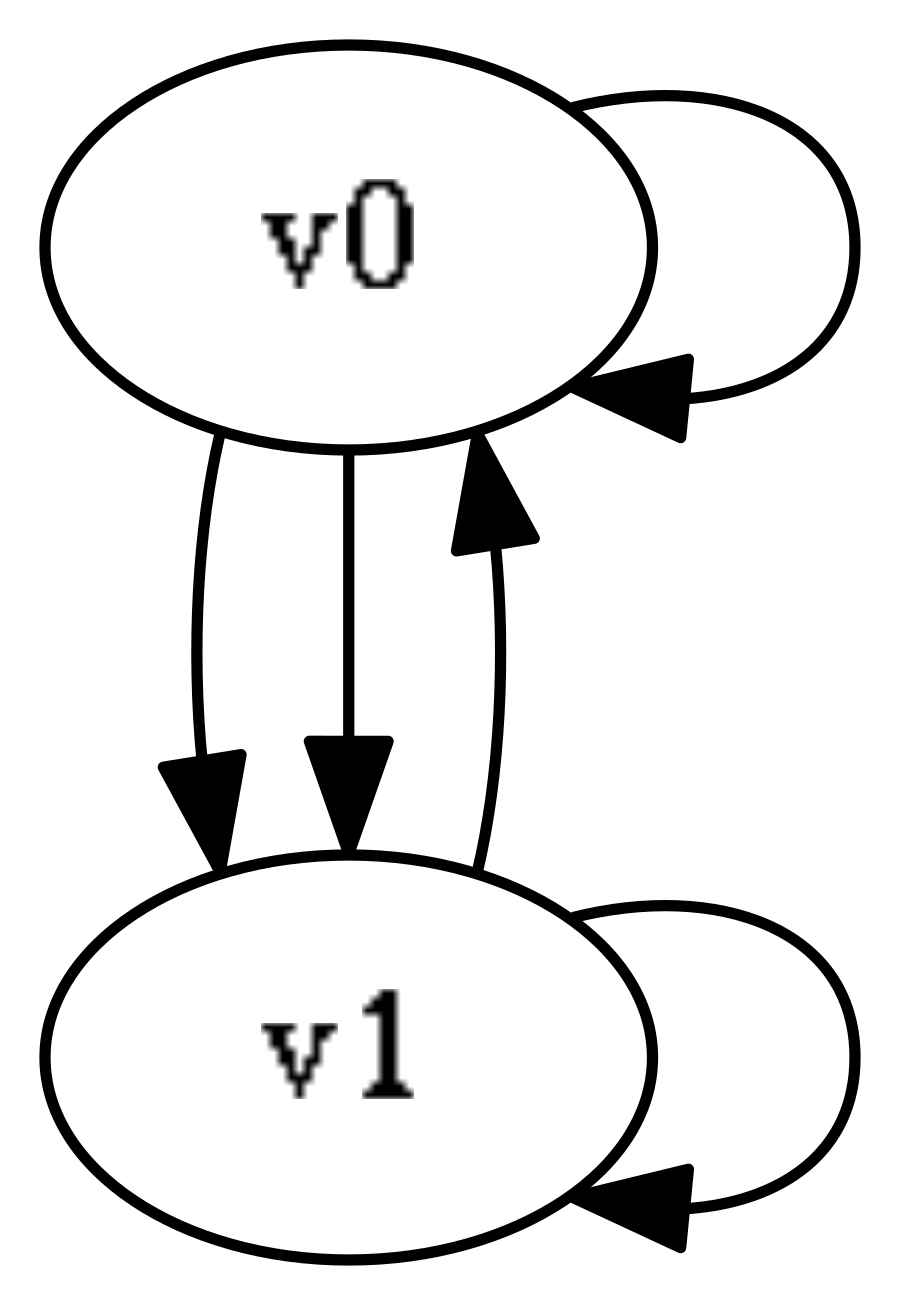
\includegraphics[height=3cm]{pic/2v_graph.png}
  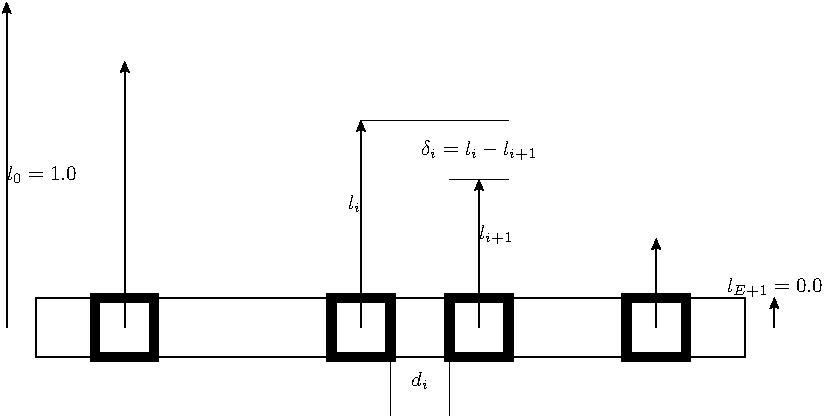
\includegraphics[height=5cm]{pic/edges.pdf}
 \end{frame}
 
  \begin{frame}{Плотный граф}
  \begin{itemize}
   \item Фаза -- период работы алгоритма без изменения фитнеса.
   \item Вероятность конца фазы: $\frac{1}{4E} \sum_{i = 0}^f d_i \delta_i$.
   \item Вероятность изменения какой-либо $\delta_i$: $\sum_{i = 1}^f (\delta_{i - 1} + \delta_i)$ 
  \end{itemize}
 \end{frame}
 
 \begin{frame}{Плотный граф}
  Уравнение для матожидания времени фазы:
  $$T(\{d_i\}_{i = 0}^f, \{\delta_i\}_{i = 0}^f) =  \sum_{i = 0}^f \frac{1}{4E}d_i \delta_i + $$
  $$ + \sum_{i = 1}^f \frac{1}{4E} \int\limits_{0}^{\delta_i + \delta_{i - 1}} (1 + T(\{d_i\}_{i = 0}^f, \{\delta_0, ... \delta_{i-1} + \delta_i - l, l, ...\delta_f\}) ) dl + $$
  $$ + \left(1 - \sum_{i = 0}^f \frac{1}{4E}d_i \delta_i - \sum_{i = 1}^f \frac{1}{4E}(\delta_{i - 1} + \delta_i) \right)(1 + T(\{d_i\}_{i = 0}^f, \{\delta_i\}_{i = 0}^f))$$
 \end{frame}
 
 \begin{frame}
  \begin{itemize}
   \item $T(\{d_i\}_{i = 0}^f, \{\delta_i\}_{i = 0}^f) = \frac{4E + \sum_{i = 1}^f\int\limits_{0}^{\delta_i + \delta_{i - 1}} (T(\{d_i\}_{i = 0}^f, \{\delta_0, ... l ...\delta_f\}) ) dl}{\sum_{i = 0}^f d_i \delta_i + \sum_{i = 1}^f (\delta_{i - 1} + \delta_i)}$
   \pitem $f = 0$:
   $$T(\{E\}, \{1\}) = 4$$
   \pitem $f = 1$:
   $$T(\{d_0, d_1\}, \{\delta_0, \delta_1\}) = \frac{4E(d_0 - d_1)}{(d_0\delta_0 + d_1\delta_1 + 1)((d_0 - d_1) - \ln\frac{d_0 + 1}{d_1 + 1})}$$
   \pitem $\delta_0 = 1$, $d_0 = 0$:
   $$T_\text{worst} = 4E \frac{E - 1}{E - 1 - \ln E}$$
  \end{itemize}
 \end{frame}

 
 \section{Эксперименты}
 \subsection{Разреженный граф}
 \begin{frame}{Разреженный граф}
  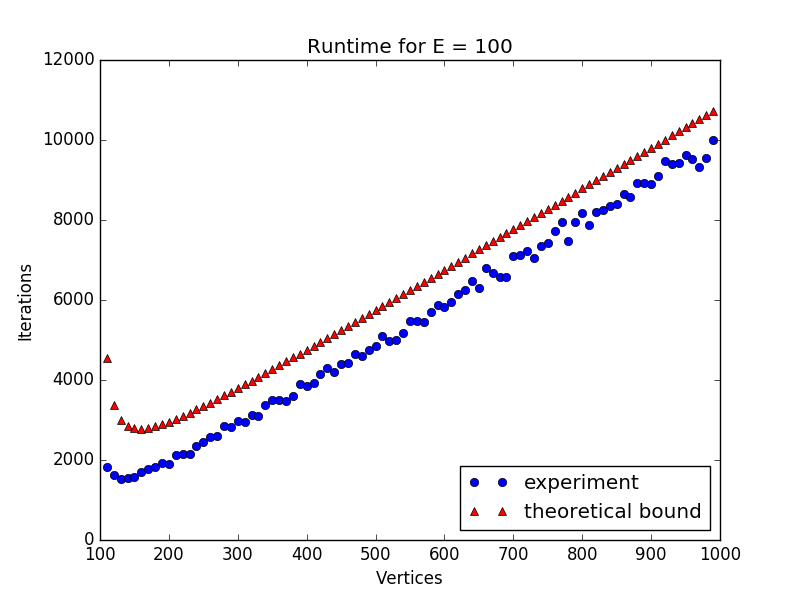
\includegraphics[width=10cm]{pic/rarefied_graph.png}
 \end{frame}
 
 \subsection{Плотный граф}
 \begin{frame}{Плотный граф}
   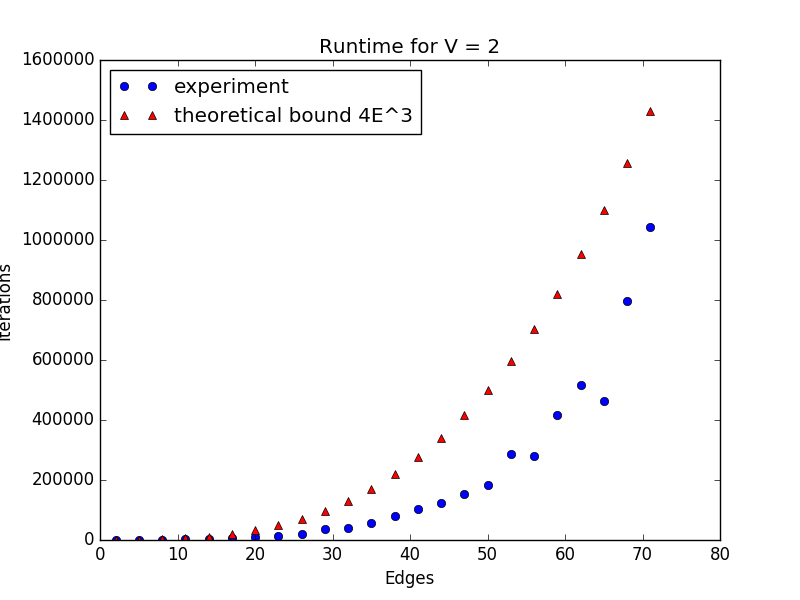
\includegraphics[width=10cm]{pic/dense_graph.png}
 \end{frame}
 
 \section{Заключение}
 \begin{frame}{Дальнейшая работа}
   \begin{itemize}
    \item Решить системы дифференциальных уравнений для $f \ge 2$
    \item Расширить рассуждение на графы с более, чем двумя вершинами.
   \end{itemize}
 \end{frame}
 
 \begin{frame}
  \begin{center}
   \Huge Спасибо!
  \end{center}

 \end{frame}


\end{document}